\documentclass[10pt,aspectration=169]{beamer}
\usepackage{graphicx}
\usepackage{subcaption} % Add the subcaption package for subfigures
\usepackage{hyperref} % Make sure hyperref is loaded after other packages


\usetheme{Warsaw}
\title[CT-Images]{RECONSTRUCTION D'IMAGES ISSUES DE TOMODENSITOMÉTRIE}
\author[Frédéric]{Frédéric ANDRIANARIVONY}
\institute[ESPA Vontovorona]{Département Éléctronique}
\date{\today}

\setbeamertemplate{navigation symbols}{} %Hiding navigation bar at the bottom
\setbeamertemplate{headline}{} %Hiding navigation bar at the top
\setbeamertemplate{frametitle continuation}{}
\setbeamercovered{transparent}


\AtBeginSection[]
{
  \begin{frame}
    \tableofcontents[currentsection]
  \end{frame}
}

\AtBeginSubsection[]
{
  \begin{frame}
    \tableofcontents[currentsection,subsectionstyle=show/shaded/hide]
  \end{frame}
}


\begin{document}
	
    \begin{frame}
        \titlepage
    \end{frame}

    \begin{frame}{Table des Matières}
        \tableofcontents
    \end{frame}

\section{Introduction}
\subsection{Enjeux de l'imagerie CT interventionnelle}
\begin{frame}{Enjeux de l'imagerie CT interventionnelle}
    \transfade
    \begin{block}<1->{Context}
        \begin{itemize}
            \item CT-scan : outil clé pour le guidage interventionnel
            \item Risque : exposition aux radiations
        \end{itemize}
    \end{block}
    \begin{block}<2->{Problématique}
        \begin{itemize}
            \item Réduction du temps d'exposition
            \item Maintien de la qualité diagnostique
        \end{itemize}
    \end{block}
    \begin{block}<3->{Solution}
        \begin{itemize}
            \item Optimiser l'acquisition des données
            \item Réduire la dose patient
            \item Garantir une image exploitable
        \end{itemize}
    \end{block}
\end{frame}

\section{Reconstruction d'images}
\subsection{Acquistion d'images}
\begin{frame}{Acquisition d'images}
    % Première image
    \only<1>{
        \begin{block}{Système de vision humaine}
            \begin{figure}
                \centering
                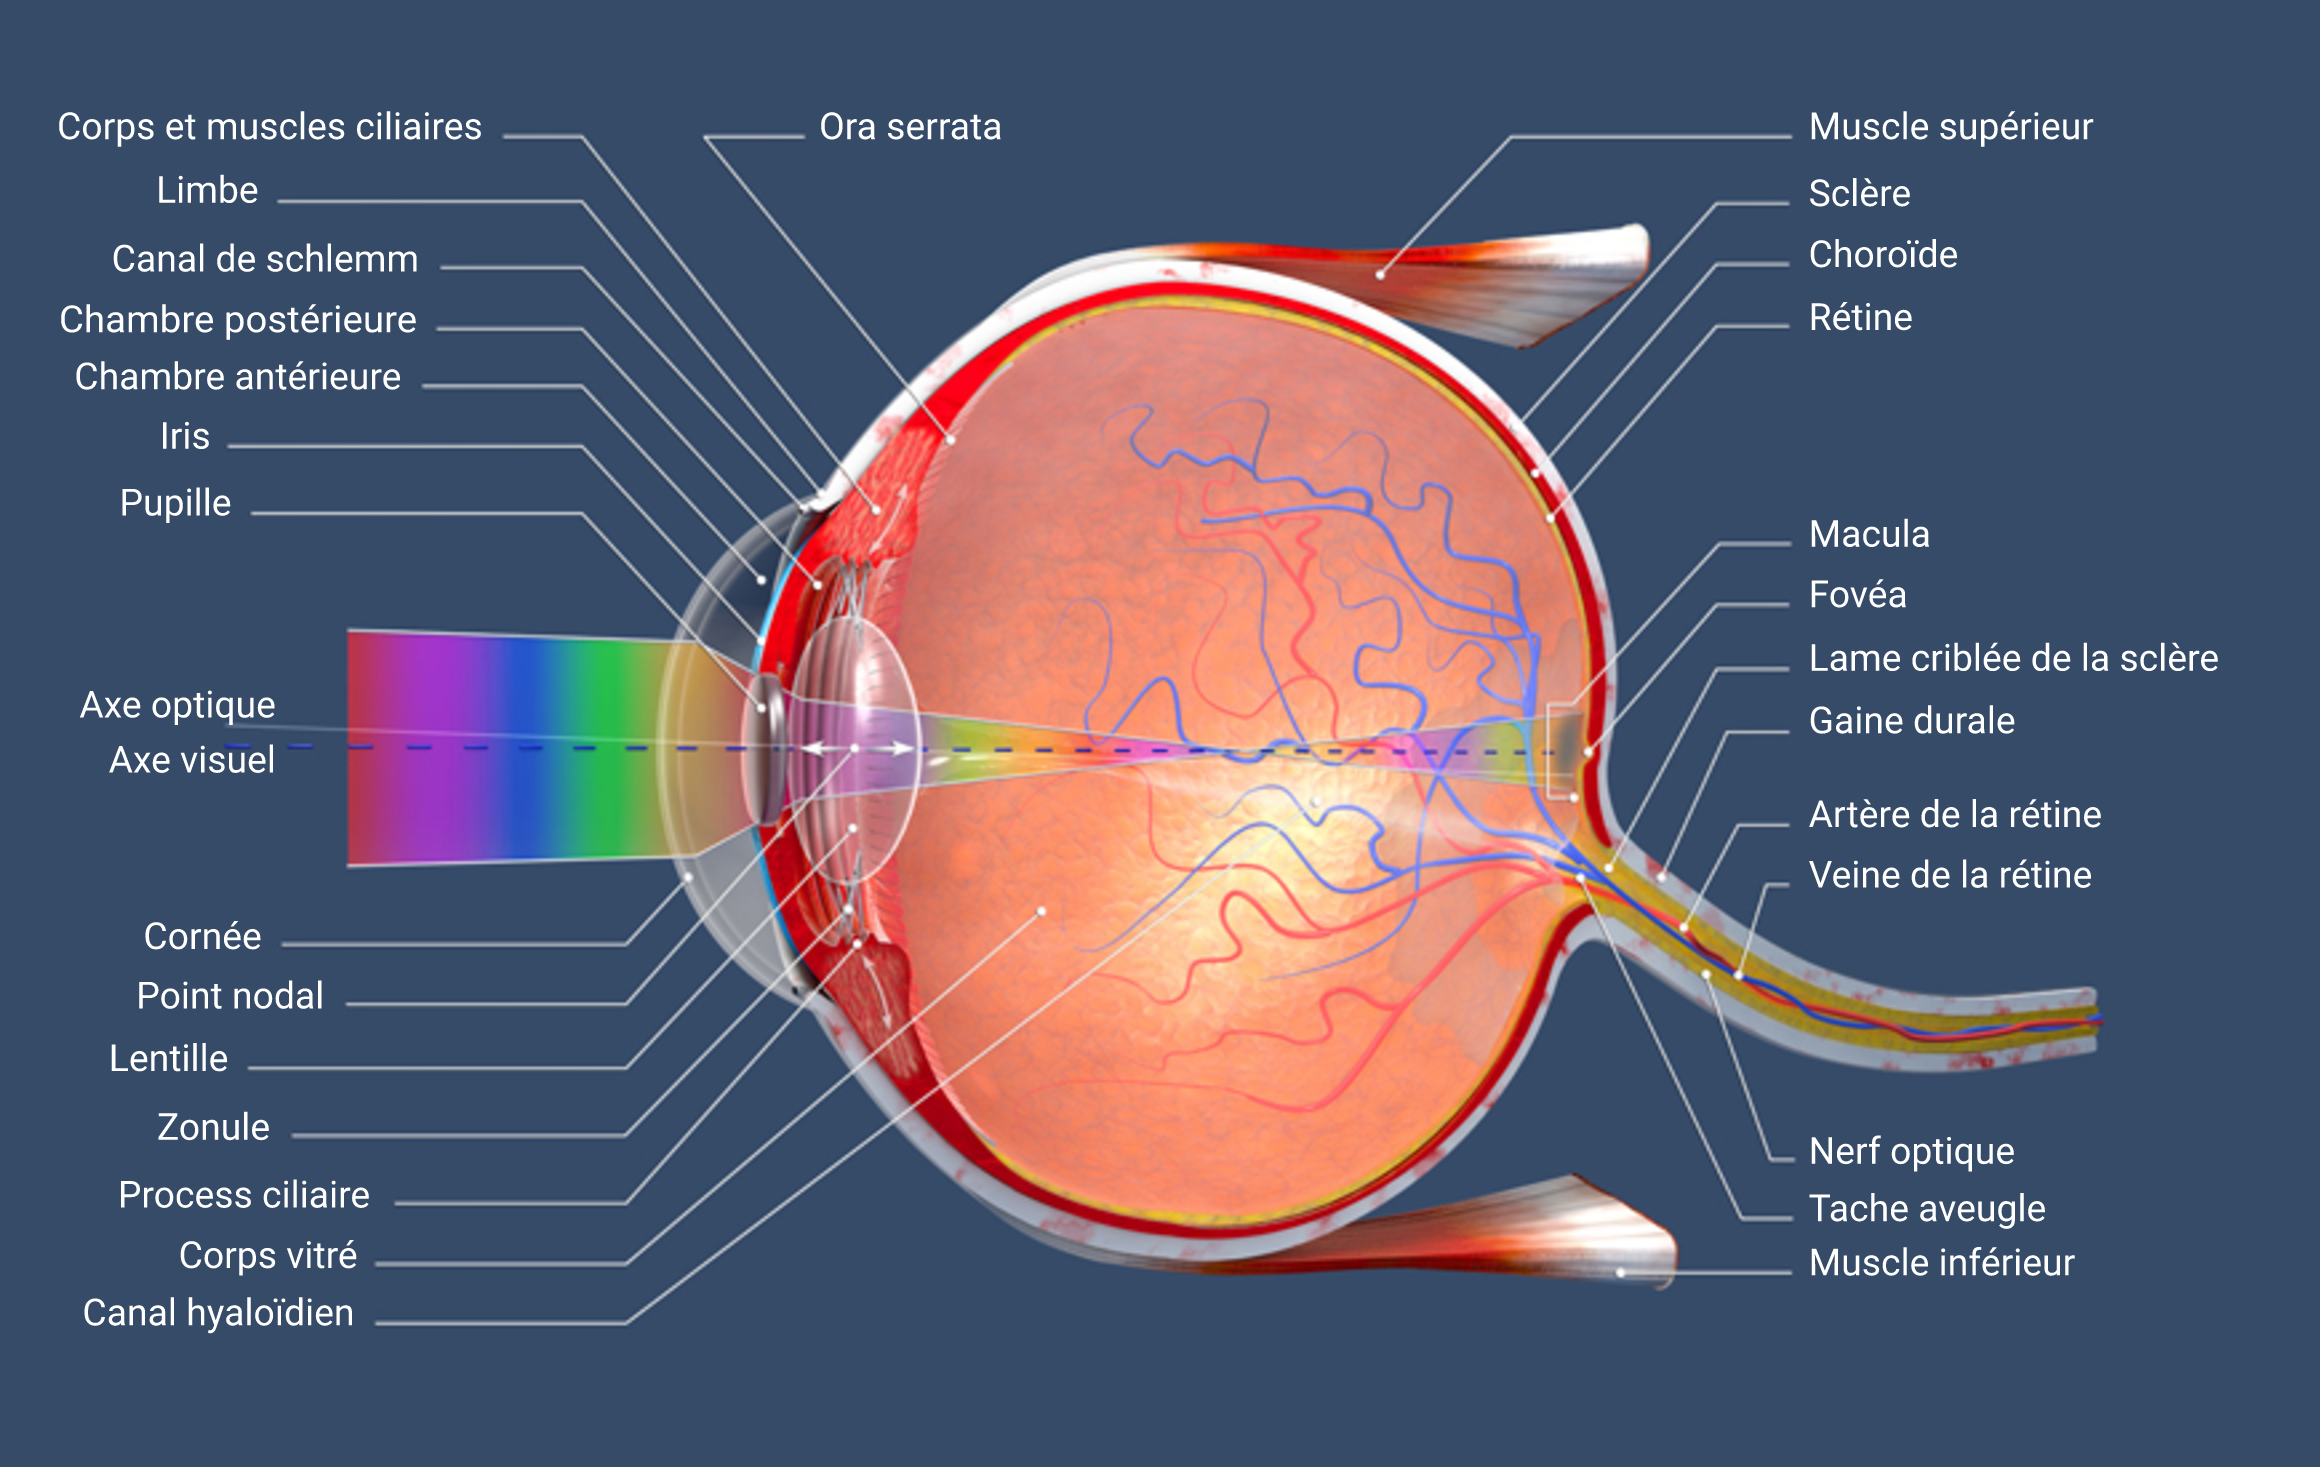
\includegraphics[width=0.6\textwidth]{../images/eye.png}
                \caption{Anatomie de l'œil humain}
                \label{fig:eye_human}
            \end{figure}
        \end{block}
    }
    % Deuxième image
    \only<2>{
        \begin{block}{Acquisition d'images analogique}
            \begin{figure}
                \centering
                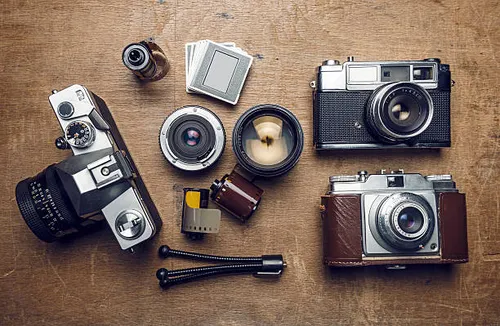
\includegraphics[width=0.6\textwidth]{../images/analog_photo.png}
                \caption{Photographie argentique -- appareils photo analogiques}
                \label{fig:analog_photo}
            \end{figure}
        \end{block}
    }
    % Troisième image
    \only<3>{
        \begin{block}{Acquisition d'images numérique}
            \begin{figure}
                \centering
                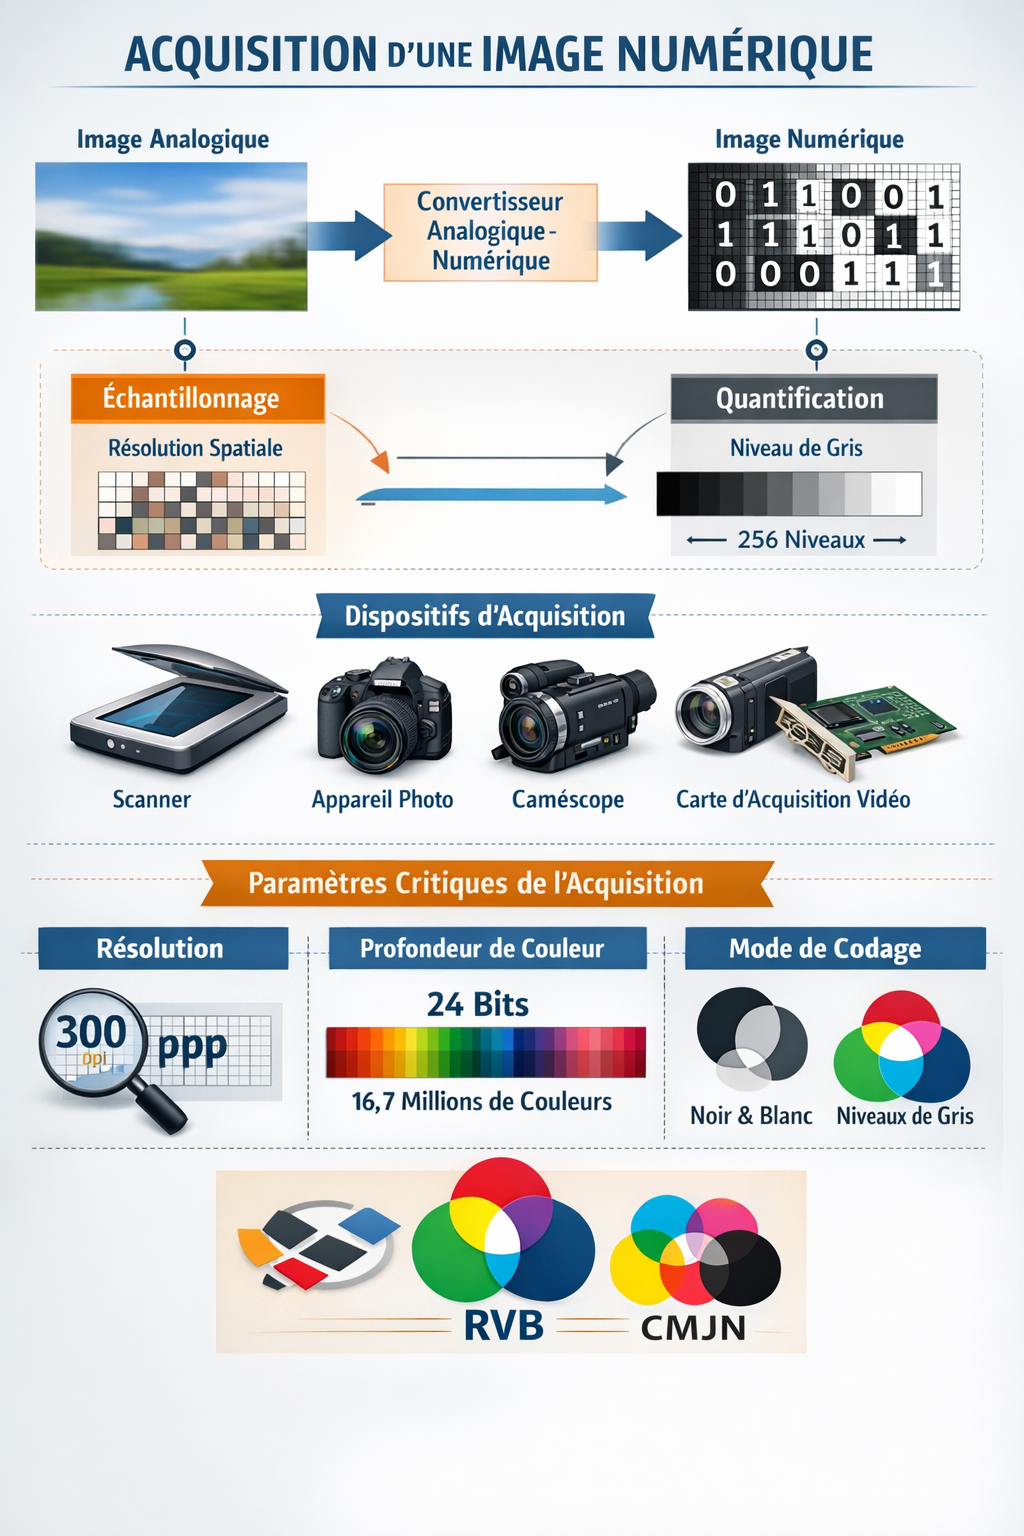
\includegraphics[height=6cm, keepaspectratio]{../images/numerical_image.png}
                \caption{Image numérique}
                \label{fig:numeric_image}
            \end{figure}
        \end{block}
    }
\end{frame}
\subsection{Système de reconstruction}
\begin{frame}{Transformation des mesures brutes en image diagnostique}
    \begin{columns}
    \column{0.5\textwidth}
    \begin{block}{Problématique}
        \begin{itemize}
            \item Les capteurs (TDM, IRM, TEP) ne mesurent \textbf{pas directement} l'image.
            \item Les données brutes $y$ sont \textbf{partielles, indirectes et bruitées}.
            \item Objectif : estimer l'image inconnue $x$ à partir de $y$.
            $\Rightarrow$ Problème \textbf{inverse}, généralement \textbf{mal posé} (non-unicité, instabilité).
        \end{itemize}
    \end{block}

    \column{0.5\textwidth}
    \begin{block}{Modélisation mathématique}
        \begin{equation}
            y = Hx + n
        \end{equation}
        \begin{itemize}
            \item $x$ : image à reconstruire (inconnue)
            \item $H$ : opérateur direct (modélise la physique de l'acquisition)
            \item $n$ : bruit de mesure
            \item $y$ : mesures acquises (sinogramme, espace $k$, projections)
        \end{itemize}
    \end{block}
\end{columns}
\end{frame}

\subsection{Algorithmes de reconstruction}
\begin{frame}{Algorithmes de reconstruction}
% Block FBP
    \only<1>{\begin{block}<1>{Rétroprojection filtrée (FBP)}
        \begin{itemize}
            \item Basée sur la transformée inverse de Radon
            \item Rapide et largement utilisée en CT et TEP
            \item Limites et artefacts :
                \begin{itemize}
                    \item Amplification du bruit
                    \item Artefacts de stries et anneaux
                    \item Sensible aux mouvements et données incomplètes
                \end{itemize}
        \end{itemize}
    \end{block}}

    \only<2>{\begin{block}{Compressive Sensing (CS)}
        \begin{itemize}
            \item Exploite la parcimonie des images médicales
            \item Reconstruction à partir de moins de mesures → réduction dose et temps d’acquisition
            \item Algorithmes itératifs avec régularisation pour limiter bruit et artefacts
            \item Limites et artefacts :
                \begin{itemize}
                    \item Sensible au choix de la base parcimonieuse et hyperparamètres
                    \item Artefacts spécifiques : blocs, textures irrégulières, effet staircasing
                \end{itemize}
            \item Stratégies d’amélioration :
                \begin{itemize}
                    \item Optimisation du sous-échantillonnage et des acquisitions
                    \item Algorithmes itératifs avancés (ex. ADMM)
                    \item Post-traitement : filtrage, amélioration du contraste
                    \item Approches hybrides : modèles physiques + statistiques
                \end{itemize}
        \end{itemize}
    \end{block}}

\end{frame}
\section{Outils mathématiques utilisés dans la reconstruction d'images ct par le compressed sensing}
\subsection{Famille de méthodes de reconstruction}
% [Speech] La reconstruction tomographique repose sur un problème inverse : retrouver l’image à partir de ses projections ou son sinogramme
\begin{frame}{Famille de méthodes de reconstruction}
    \only<1>{
        % [Speech] Permet de determiner le coefficient d'attenuation
        \begin{columns}
            \column{0.5\textwidth}
            \begin{block}{Loi de Beer-Lambert} 
                \begin{equation}
                    I(x) = I_0 e^{-A(x)\, x}
                \end{equation}
                où \begin{itemize}
                    \item $x$ est la distance parcourue par le rayon $X$
                    \item $I(x)$ est l'intensité final 
                    \item $I_0$ est l'intensité initiale
                    \item $A(x)$ est la proportion de photons absorbés sur un distance $x$
                \end{itemize}
            \end{block}

            \column{0.5\textwidth}
            \begin{block}{Sinogramme}
                \begin{equation}
                    ln(I(x0)/I(x1)) = \int_{x0}^{x1} A(x)\, dx
                \end{equation}
                où $ln(I(x0)/I(x1))$ désigne les données de projection, communément appelées le sinogramme
            \end{block}
        \end{columns}
    }
    \only<2>{
        \begin{columns}
            \column{0.33\textwidth}
            \begin{figure}[H]
                \centering
                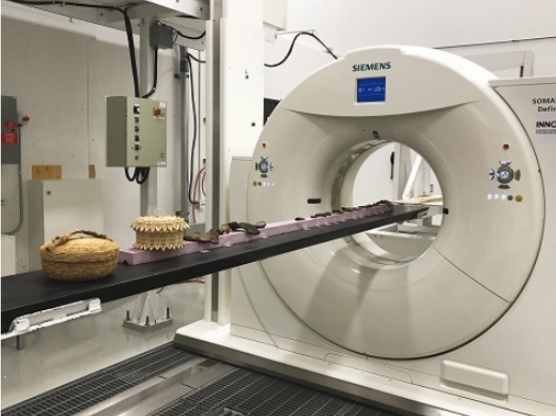
\includegraphics[height=3cm, keepaspectratio]{../images/ct_device.png}
                \caption{Appareil de tomodensitométrie}
                \label{fig :tomography_device}
            \end{figure}

            \column{0.33\textwidth}
            \begin{figure}[H]
                \centering
                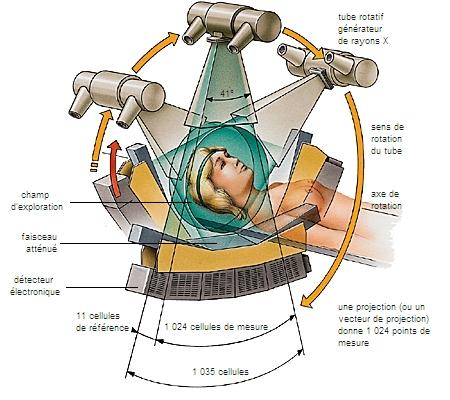
\includegraphics[height=3cm, keepaspectratio]{../images/ct_scan_operation.jpeg}
                \caption{Fonctionnement de la CT-Scan}
                \label{fig :tomography_device_operation}
            \end{figure}

            \column{0.33\textwidth}
            \begin{figure}[H]
                \centering
                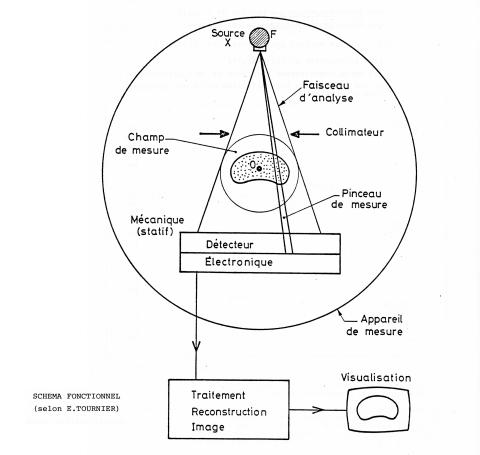
\includegraphics[height=3cm, keepaspectratio]{../images/ct_scan_reconstruction_process.jpeg}
                \caption{Processus de reconstruction}
                \label{fig :tomography_device_operation}
            \end{figure}
        \end{columns}
    }
    \only<3>{
        \begin{block}{Filter Back Projection (FBP)}
            \begin{equation}
                f(x,y) \approx \frac{1}{2}\,\mathcal{B}\!\left(\mathcal{F}^{-1} S' \star \mathcal{R}f \right)(x,y).
                \label{eq:FBP_varphi_approx}
            \end{equation}
            où \begin{itemize}
                \item $\mathcal{F}^{-1}$ est l'inverse de la transformée de Fourier
                \item $\mathcal{B}$ est la retroprojection
                \item $S'$ est un filtre filtre passe-bas
                \item $\mathcal{R}f$ est la transformée de Radon de $f$
            \end{itemize}
        \end{block}
    }
    \only<4>{
        \begin{block}{Approches discrète}
            \begin{equation}
                g=Af
            \end{equation}
            où \begin{itemize}
                    \item $A$ (matrice système) représente la transformée de Radon discrète
                    \item $g$ est le sinogramme mesuré
                    \item $f$ est l'image à reconstruire
            \end{itemize}
        \end{block}
    }\only<4>{
        % [Speech] Un signal peut être reconstruit à partir de très peu de mesures s'il est parcimonieux dans un domaine de représentation adapté.
        \begin{block}{Compressive Sensing (CS)}
            \begin{equation}
                \min_f ||A f - g||^2 + \lambda \Phi(f)
            \end{equation}
                où $\Phi(f)$ = régularisation (sparsité)

        \end{block}
    }
    \only<5>{
        \begin{figure}[H]
            \centering
            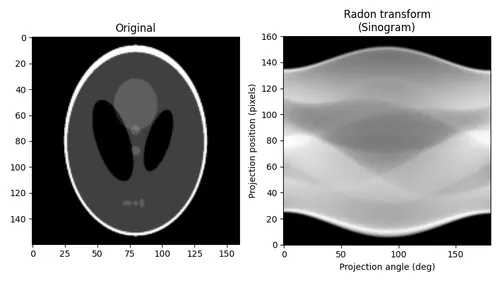
\includegraphics[height=3cm, keepaspectratio]{../images/sinogram_and_reconstructed_image.png}
            \caption{Pair image-sinogramme}
            \label{fig :tomography_device_operation}
        \end{figure}
    }
\end{frame}

\section{Approche ADMM associée aux ondelettes biorthogonales 4.4}

\subsection{Problème inverse en tomodensitométrie}
\begin{frame}{Modélisation du problème}
        \begin{equation}
            \mathbf{g} = A \mathbf{f} + \mathbf{n}
        \end{equation}
        où \begin{itemize}
            \item \( \mathbf{f} \) : image (coefficients d'atténuation)
            \item \( \mathbf{g} \) : projections (sinogramme)
            \item \( A \) : transformée de Radon discrète
            \item \( \mathbf{n} \) : bruit
        \end{itemize}
\end{frame}

\subsection{Mal-positude}
\begin{frame}{Mal-positude}
    \transfade
    \begin{block}<1->{Difficulté de la reconstruction}
        \begin{itemize}
            \item Sous-déterminé
            \item Sensible au bruit
            \item Non unicité des solutions
        \end{itemize}
    \end{block}

    \begin{block}<2->{Conséquences}
        \begin{itemize}
            \item artefacts
            \item instabilité
            \item mauvaise qualité image
        \end{itemize}
    \end{block}
\end{frame}

\subsection{Ondelettes orthogonales}
\begin{frame}{Ondelettes orthogonales}

    \textbf{Principe fondamental}
    \begin{itemize}
        \item La base d'analyse et la base de synthèse coïncident
        \item L'opérateur de transformation $W$ est une matrice orthogonale
    \end{itemize}

    \textbf{Propriétés mathématiques}
    \begin{itemize}
        \item L'adjoint coïncide avec l'inverse :
        \[
        W^T = W^{-1}
        \]
        \item Orthogonalité des colonnes :
        \[
        W^T W = I
        \]
        \item Conservation de l'énergie (propriété de Parseval) :
        \[
        \|Wx\|_2 = \|x\|_2
        \]
        \item Représentation non redondante : $m = n$
    \end{itemize}
    % \textbf{Avantages et limitations}
    % \begin{itemize}
    %     \item[+] Conservation exacte de l'énergie
    %     \item[+] Reconstruction parfaite et simple ($W^{-1} = W^T$)
    %     \item[+] Transformation bijective et sans redondance
    %     \item[-] Filtres généralement non symétriques
    %     \item[-] Absence de phase linéaire (distorsion possible des contours)
    % \end{itemize}
    \textbf{Exemples :} Haar, Daubechies, Symlets

\end{frame}


\subsection{Ondelettes biorthogonales}
\begin{frame}{Ondelettes biorthogonales}
    \textbf{Principe fondamental}
    \begin{itemize}
        \item Deux bases distinctes :
        \begin{itemize}
            \item Base d'analyse : $W$ (décomposition)
            \item Base de synthèse : $\tilde{W}$ (reconstruction)
        \end{itemize}
        \item Filtres d'analyse : $h$, $g$ (passe-bas, passe-haut)
        \item Filtres de synthèse : $\tilde{h}$, $\tilde{g}$ (passe-bas, passe-haut)
    \end{itemize}

    \vspace{0.2cm}

    \textbf{Propriétés mathématiques}
    \begin{itemize}
        \item Reconstruction parfaite :
        \[
        \tilde{W} W = I
        \]
        \item L'adjoint de l'analyse n'est pas l'opérateur de synthèse :
        \[
        W^T \neq \tilde{W}
        \]
        \item Condition de biorthogonalité :
        \[
        \langle \psi_{j,k}, \tilde{\psi}_{j',k'} \rangle = \delta_{j,j'} \delta_{k,k'}
        \]
    \end{itemize}

    % \vspace{0.2cm}

    % \textbf{Avantages pratiques}
    % \begin{itemize}
    %     \item[+] Filtres symétriques possibles → phase linéaire
    %     \item[+] Meilleure préservation des contours et structures géométriques
    %     \item[+] Flexibilité accrue dans la conception des filtres
    %     \item[+] Qualité de reconstruction supérieure pour l'imagerie
    % \end{itemize}

    % \vspace{0.2cm}

    % \textbf{À retenir pour l'optimisation}
    % \begin{itemize}
    %     \item Reconstruction effective : $\tilde{W}$ (synthèse)
    %     \item Gradient / optimisation : $W^T$ (adjoint mathématique)
    %     \item \textcolor{red}{Attention :} Certaines implémentations utilisent $\tilde{W}$ à la place de $W^T$
    % \end{itemize}

    % \vspace{0.2cm}
    \textbf{Exemples :} Bior4.4, Bior2.2, Bior6.8

\end{frame}

\subsection{Reconstruction tomographique à faible dose par parcimonie: Compressed Sensing}
\begin{frame}{Modélisation CT et exploitation de la parcimonie}
    \transfade
    \only<1>{\begin{block}{Modèle d'acquisition CT}
        \begin{equation}
            \mathbf{g} = A \mathbf{f} \in \mathbb{R}^m, \quad A \in \mathbb{R}^{m \times n} \text{ (matrice système)}
        \end{equation}
        \begin{itemize}
            \item $\mathbf{f} \in \mathbb{R}^n$ : image à reconstruire
            \item $\mathbf{g} \in \mathbb{R}^m$ : projections (sinogramme)
            \item $A$ : modélise la géométrie CT
        \end{itemize}
    \end{block}}

    \only<2>{\begin{block}{Avec représentation parcimonieuse}
        \begin{equation}
            \mathbf{g} = A \mathbf{f} = A W \mathbf{x} = \Phi' \mathbf{x}, \quad \Phi' = A W
        \end{equation}
        \begin{itemize}
            \item $W$ : matrice d'ondelettes
            \item $\mathbf{x}$ : coefficients parcimonieux dans la base $W$
            \item $\Phi'$ : matrice combinée système CT + ondelettes
        \end{itemize}
        \vspace{0.5em}
        \centering
        \textit{On travaille maintenant directement avec les coefficients parcimonieux $\mathbf{x}$ pour reconstruire $\mathbf{f}$ à partir de peu de mesures.}
    \end{block}}

\end{frame}

\subsection{Approche ADMM combinée avec ondelettes (Bior4.4)}
\begin{frame}{ADMM combinée à bior4.4}
    \transfade
    \only<1>{\begin{block}{Principe ADMM}
        Décomposition du problème
        On introduit :
        \[
        z = W\mathbf{f}
        \]
        
        \[
        \min_{\mathbf{f},z}
        \frac{1}{2} ||A\mathbf{f} - \mathbf{g}||_2^2 + \lambda ||z||_1
        \]
    \end{block}}
    \only<2>{\begin{block}{Lagrangien augmenté}
        \[
        L_\rho(\mathbf{f},z,u) =
        \frac{1}{2} ||A\mathbf{f} - \mathbf{g}||_2^2
        + \lambda |z|_1
        + \frac{\rho}{2} ||W\mathbf{f} - z + u||_2^2
          \]
    \end{block}
    où \begin{itemize}
            \item $\mathbf{x}$ : variable primaire, vecteur des coefficients d'image à reconstruire
            \item $z$ : variable auxiliaire pour séparer le terme $\ell_1$ et faciliter l'optimisation
            \item $u$ : variable duale mise à l'échelle (dual scaled), associée à la contrainte $Wx = z$
            \item $W$ : matrice de transformation (par exemple, base d'ondelettes ou opérateur de gradient)
            \item $A$ : opérateur de mesure (matrice système ou projection CT)
            \item $\mathbf{y}$ : vecteur de mesures (sinogramme)
            \item $\lambda$ : paramètre de régularisation, contrôle l'importance de la parcimonie
            \item $\rho > 0$ : paramètre de pénalité, contrôle l'écart à la contrainte $Wx = z$ et influence la vitesse de convergence
        \end{itemize}
    }
    \only<3>{
    \begin{block}{Algorithme ADMM}
        \begin{itemize}
            \item \textbf{Mise à jour de $\mathbf{x}$ (sous-problème quadratique)}  
            Résolution du système :
            \[
            x^{k+1} = \arg\min_{x} \frac{1}{2}\|\mathcal{A}x - y\|_2^2 + \frac{\rho}{2}\|Wx - z^k + u^k\|_2^2
            \]
            ou équivalent linéaire :
            \[
            (A^T A + \rho W^T W)x = A^T y + \rho W^T (z^k - u^k)
            \]

            \item \textbf{Mise à jour de $z$ (seuillage doux)}  
            Imposition de la parcimonie via l’opérateur proximal $\ell_1$ :
            \[
            z^{k+1} = \mathcal{S}_{\lambda / \rho}(Wx^{k+1} + u^k), \quad
            \mathcal{S}_{\tau}(t) = \operatorname{sign}(t)\max(0, |t|-\tau)
            \]

            \item \textbf{Mise à jour de la variable duale $u$}  
            Correction de la violation de contrainte $Wx = z$ :
            \[
            u^{k+1} = u^k + (Wx^{k+1} - z^{k+1})
            \]
        \end{itemize}
    \end{block}}
\end{frame}

\section{Reconstruction tomographique parcimonieuse par ADMM et ondelettes Bior4.4}
%------------------------------------------------
\begin{frame}{Résultats Quantitatifs}
    \only<1>{
        \begin{block}{Performance de la méthode ADMM-Bior4.4}
            \textbf{Cas d'étude détaillé (Image Shepp-Logan)}
            \begin{table}[H]
            \centering
            \caption{Évaluation comparative des performances de reconstruction}
            \label{tab:quantitative_results}
            \begin{tabular}{lcc}
            \hline
            \textbf{Méthode} & \textbf{PSNR $\uparrow$ (dB)} & \textbf{SSIM $\uparrow$}  \\
            \hline
            FBP & 25.04 & 0.678 \\
            ISTA & 24.83 & 0.768  \\
            FISTA & 31.50 & 0.758  \\
            ADMM-Bior4.4 & \textbf{37.31} & \textbf{0.972}  \\
            \hline
            \end{tabular}
            \end{table}
            
            \begin{itemize}
                \item Ces valeurs, obtenues sur l'image de référence, démontrent une reconstruction de très haute qualité, avec une excellente préservation des structures anatomiques.
            \end{itemize}
        \end{block}
    }
    % \only<2>{
    %     \begin{block}{Performances moyennes sur l'ensemble des 19 images}
    %         \begin{table}[h]
    %         \centering
    %         \caption{Comparaison des métriques PSNR et SSIM}
    %         \begin{tabular}{|c|c|c|c|c|}
    %         \hline
    %         \textbf{Algorithme} & \textbf{PSNR\_mean} & \textbf{PSNR\_std} & \textbf{SSIM\_mean} & \textbf{SSIM\_std} \\
    %         \hline
    %         ADMM-Bior4.4 & 26.203727 & 0.151281 & 0.865829 & 0.008924 \\
    %         FISTA         & 25.132216 & 0.220781 & 0.677443 & 0.010547 \\
    %         ISTA          & 22.397596 & 0.385292 & 0.650520 & 0.015583 \\
    %         FBP           & 21.610267 & 0.301994 & 0.558846 & 0.021965 \\
    %         \hline
    %         \end{tabular}
    %         \end{table}
    %     \end{block}
    % }
    \only<2>{
        \begin{block}{Performances moyennes sur l'ensemble des 19 images}
            \centering
            \captionof{table}{Comparaison des métriques PSNR et SSIM}
            \resizebox{0.9\textwidth}{!}{
                \begin{tabular}{|c|c|c|c|c|}
                \hline
                \textbf{Algorithme} & \textbf{PSNR\_mean} & \textbf{PSNR\_std} & \textbf{SSIM\_mean} & \textbf{SSIM\_std} \\
                \hline
                ADMM-Bior4.4 & 26.203727 & 0.151281 & 0.865829 & 0.008924 \\
                FISTA         & 25.132216 & 0.220781 & 0.677443 & 0.010547 \\
                ISTA          & 22.397596 & 0.385292 & 0.650520 & 0.015583 \\
                FBP           & 21.610267 & 0.301994 & 0.558846 & 0.021965 \\
                \hline
                \end{tabular}%
            }
        \end{block}
    }
    \only<3>{
        \begin{block}{Analyse et Interprétation}
            \begin{itemize}
                \item \textbf{Analyse :} ADMM-Bior4.4 surpasse nettement les autres méthodes en moyenne, avec des écarts-types plus faibles, attestant d'une grande stabilité.
                
                \vspace{0.3cm}
                
                \item \textbf{Interprétation :}
                \begin{itemize}
                    \item Un \textbf{PSNR} de 26.20 dB indique une excellente fidélité aux données.
                    \item Un \textbf{SSIM} de 0.866, proche de 1, confirme une très bonne préservation des structures anatomiques, même en contexte de sous-échantillonnage.
                \end{itemize}
            \end{itemize}
        \end{block}
    }
\end{frame}

	\bibliographystyle{unsrt}
    \begin{thebibliography}{100}
        \bibitem{17} \emph{Comparison between orthogonal and bi-orthogonal wavelets}
        \bibitem{14}  Engl, Heinz W., and R. Ramlau, \emph{Regularization of inverse problems}. Kluwer Academic Publishers, 2000.
        \bibitem{9} Jen Beatty Colby College, \emph{The Radon Transform and the Mathematics of Medical Imaging}
        \bibitem{10} R. Snieder and J. Trampert. \emph{Linear and nonlinear inverse problems}. Department of Geophysics, Utrecht University, P.O. Box 80.021, 3508 TA Utrecht, The Netherlands. Email: snieder@geo.uu.nl.
        \bibitem{11} I. Bloch. \emph{Reconstruction d’images de tomographie}. LTCI, Télécom Paris, Isabelle.Bloch@telecom-paris.fr.
        \bibitem{12} S. Qin. \emph{Simple algorithm for L1-norm regularisation-based compressed sensing and image restoration}. Third Institute of Physics, Georg-August-Universität Göttingen, Friedrich-Hund-Platz 1, Göttingen, Germany. Email: shun.qin@outlook.com.
        \bibitem{13} M. Piening, F. Altekrüger, J. Hertrich, P. Hagemann, A. Walther and G. Steidl. \emph{Learning from small data sets: Patch-based regularizers in inverse problems for image reconstruction}. (Information manquante pour l’affiliation complète). Note: Les affiliations sont indiquées par les chiffres 1 et 2, mais ne sont pas détaillées dans le texte fourni.
        \bibitem{15} Stephen Boyd , Neal Parikh , Eric Chu Borja Peleato and Jonathan Eckstein \emph{Distributed Optimization and Statistical Learning via the Alternating Direction Method of Multipliers}
        \bibitem{18}CANDITIIS, D.D. and VIDAKOVIC, B. (2004) \emph { Wavelet Bayesian Block Shrinkage via Mixtures of Normal-Inverse Gamma Priors}. Journal of Computational and Graphical Statistics, 13 (2), pp. 383-398
        \bibitem{19} LIU, C.-L. (2010) \emph{A Tutorial of the Wavelet Transform}.
        
        \bibitem{20}MEEN, R.S. and SHARMA, A. (2014) \emph{Comparison and Analysis of Orthogonal and Biorthogonal Wavelets for ECG Compression}. International Journal of Research in Engineering and Technology, 3 (3), pp. 242-247.
        \bibitem{21} WIM SWELDENS \emph{THE LIFTING SCHEME: A CONSTRUCTION OF SECOND GENERATION WAVELETS}

        \bibitem{22} Y. Wang, Z. Liu, and H. Chen, \emph{Accurate Image Quality Assessment in Compressive Sensing: Beyond PSNR and MSE}, IEEE Transactions on Image Processing, vol. 33, pp. 2105--2118, 2024. DOI: 10.1109/TIP.2024.3372109.

      \bibitem{23} A. Gupta and R. Singh, \emph{Efficient Error Metrics for Sparse Signal Recovery in Medical Imaging}, Signal Processing, vol. 212, pp. 109145, 2023. DOI: 10.1016/j.sigpro.2023.109145.

      \bibitem{24} Y. Liu, H. Zhang, and Q. Wang, \emph{High-Fidelity Image Recovery in Compressive Sensing: A PSNR-Driven Optimization Framework}, IEEE Transactions on Multimedia, 2024.

      \bibitem{25} W. Simoes and M. De Sa, \emph{PSNR and SSIM: Evaluation of the Imperceptibility Quality of Images Transmitted over Wireless Networks}, Procedia Computer Science, 2024. DOI: 10.1016/j.procs.2024.11.134.


      \bibitem{26} Z. Wang and A. C. Bovik, \emph{Advances in Structural Similarity Metrics for Image Quality Assessment}, IEEE Transactions on Pattern Analysis and Machine Intelligence, vol. 45, no. 8, pp. 10212--10227, 2023. DOI: 10.1109/TPAMI.2023.3267890.

      \bibitem{27} H. Li, Y. Liu, and J. Zhang, \emph{SSIM-Based Optimization for Compressive Sensing Reconstruction in Medical Imaging}, Medical Image Analysis, vol. 92, pp. 102987, 2024. DOI: 10.1016/j.media.2023.102987.
      \bibitem{28} Jonathan Richard Shewchuk \emph{An Introduction to the Conjugate Gradient Method Without the Agonizing Pain}
      \bibitem{29} Jeremy E. Cohen \emph{Computing the proximal operator of the $\ell_1$ induced matrix norm}
    \end{thebibliography}
\end{document}
